%%%%%%%%%%%%%%%%%%%%%%%%
%
% $Autor: Hemanth Jadiswami Prabhakaran $
% $Datum: 2025-06-30 11:18:33Z $
% $Pfad: GitHub/BA25-01-Time-Series/Manual/Chapters/en/02InstallationAndSetup.tex $
% $Version: 1 $
%
% $Project: BA25-Time-Series $
%
%%%%%%%%%%%%%%%%%%%%%%%%



\chapter{Installation and Setup}

\section{Deployment Options Overview}

The Walmart Sales Forecasting System offers two deployment methods to accommodate different user needs and technical environments. Each option provides full system functionality with specific advantages for different use cases.

\begin{figure}[H]
    \centering
    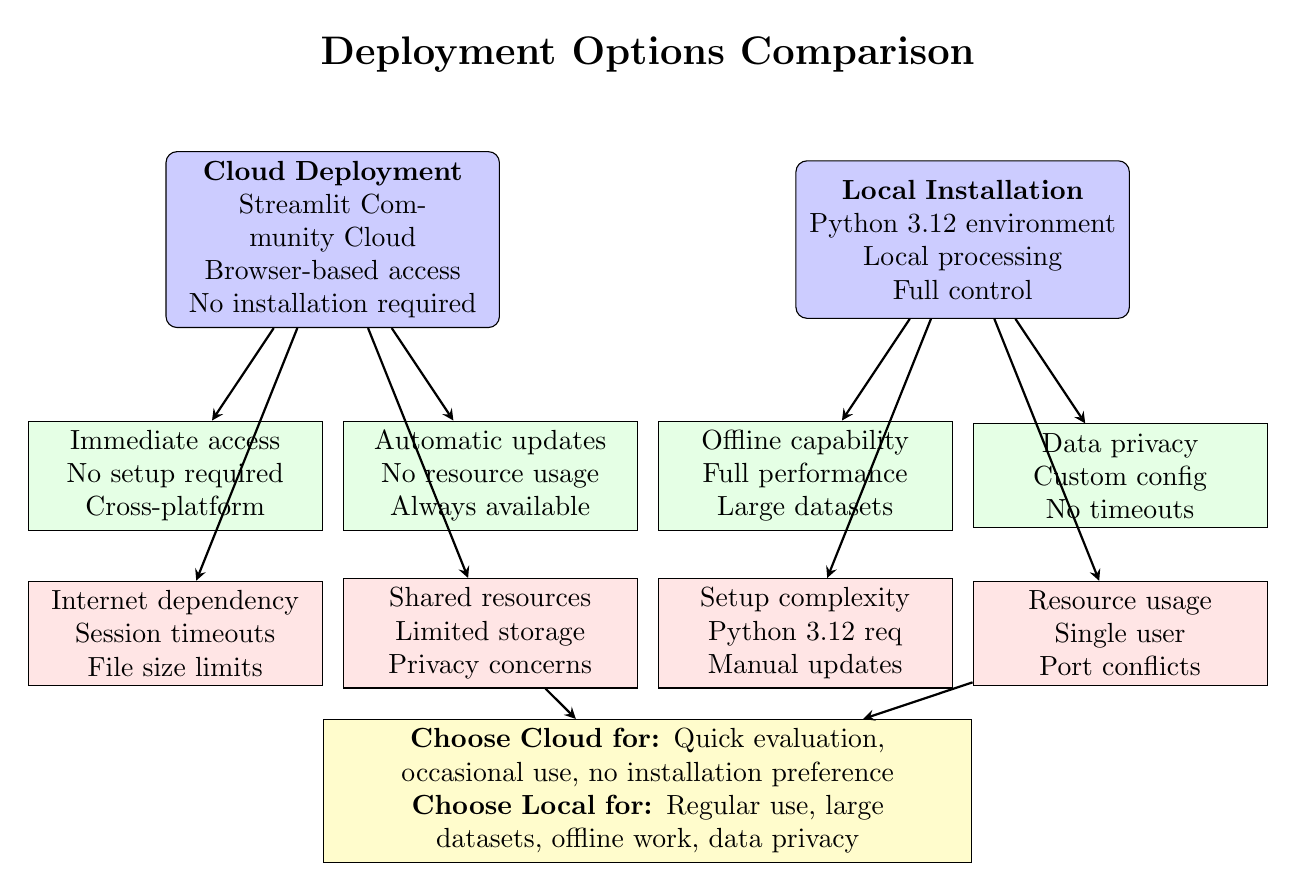
\begin{tikzpicture}[
    node distance=2.5cm,
    option/.style={rectangle, draw, fill=blue!20, text width=4cm, text centered, rounded corners, minimum height=2cm},
    pro/.style={rectangle, draw, fill=green!10, text width=3.5cm, text centered, minimum height=1cm},
    con/.style={rectangle, draw, fill=red!10, text width=3.5cm, text centered, minimum height=1cm},
    arrow/.style={thick,->,>=stealth}
]

% Title
\node[above=2cm] at (0,0) {\Large\textbf{Deployment Options Comparison}};

% Main options
\node[option] (cloud) at (-4,0) {\textbf{Cloud Deployment}\\Streamlit Community Cloud\\Browser-based access\\No installation required};

\node[option] (local) at (4,0) {\textbf{Local Installation}\\Python 3.12 environment\\Local processing\\Full control};

% Cloud advantages
\node[pro] (cloud_pro1) at (-6,-3) { Immediate access\\ No setup required\\ Cross-platform};
\node[pro] (cloud_pro2) at (-2,-3) { Automatic updates\\ No resource usage\\ Always available};

% Cloud disadvantages  
\node[con] (cloud_con1) at (-6,-5) { Internet dependency\\ Session timeouts\\ File size limits};
\node[con] (cloud_con2) at (-2,-5) { Shared resources\\ Limited storage\\ Privacy concerns};

% Local advantages
\node[pro] (local_pro1) at (2,-3) { Offline capability\\ Full performance\\ Large datasets};
\node[pro] (local_pro2) at (6,-3) { Data privacy\\ Custom config\\ No timeouts};

% Local disadvantages
\node[con] (local_con1) at (2,-5) { Setup complexity\\ Python 3.12 req\\ Manual updates};
\node[con] (local_con2) at (6,-5) { Resource usage\\ Single user\\ Port conflicts};

% Connecting arrows
\draw[arrow] (cloud) -- (cloud_pro1);
\draw[arrow] (cloud) -- (cloud_pro2);
\draw[arrow] (cloud) -- (cloud_con1);
\draw[arrow] (cloud) -- (cloud_con2);

\draw[arrow] (local) -- (local_pro1);
\draw[arrow] (local) -- (local_pro2);
\draw[arrow] (local) -- (local_con1);
\draw[arrow] (local) -- (local_con2);

% Decision flow
\node[rectangle, draw, fill=yellow!20, text width=8cm, text centered] (decision) at (0,-7) {
\textbf{Choose Cloud for:} Quick evaluation, occasional use, no installation preference\\
\textbf{Choose Local for:} Regular use, large datasets, offline work, data privacy
};

\draw[arrow] (cloud_con2) -- (decision);
\draw[arrow] (local_con2) -- (decision);

\end{tikzpicture}
    \caption{Deployment Options Technical Comparison}
    \label{fig:deployment_options}
\end{figure}

\section{Cloud Access (Recommended for Quick Start)}

\subsection{Immediate Browser Access}

For immediate system access without any installation requirements, use the cloud-hosted applications:

\begin{itemize}
    \item \textbf{Training Application}: \url{https://walmart-sales-training-app-py.streamlit.app/}
    \item \textbf{Prediction Application}: \url{https://walmart-sales-prediction-app-py.streamlit.app/}
\end{itemize}

\subsection{Cloud Access Procedure}

\begin{enumerate}
    \item Open a modern web browser (Chrome, Firefox, Safari, or Edge)
    \item Navigate to the desired application URL
    \item Wait for the Streamlit application to load (typically 10-30 seconds)
    \item Begin using the application immediately
\end{enumerate}

\begin{figure}[H]
    \centering
    \includegraphics[width=0.9\textwidth]{Images/02InstallationAndSetup/CloudAccess.png}
    \caption{Cloud Application Loading Interface}
    \label{fig:cloud_access}
\end{figure}

\subsection{Cloud Advantages}

\begin{itemize}
    \item \textbf{No Installation Required}: Immediate access without software setup
    \item \textbf{Cross-Platform Compatibility}: Works on any device with a web browser
    \item \textbf{Automatic Updates}: Always running the latest version
    \item \textbf{No Resource Requirements}: Server-side processing
\end{itemize}

\subsection{Cloud Limitations}

\begin{itemize}
    \item \textbf{Internet Dependency}: Requires stable internet connection
    \item \textbf{File Upload Size Limits}: Large dataset restrictions may apply
    \item \textbf{Session Timeout}: Extended idle periods may reset the application
\end{itemize}

\section{Local Installation (Advanced Users)}

\subsection{System Requirements}

Before proceeding with local installation, ensure your system meets these requirements:

\begin{itemize}
    \item \textbf{Python Version}: Exactly Python 3.12.x (not 3.12+ or other versions)
    \item \textbf{Operating System}: Windows, macOS, or Linux
    \item \textbf{Available Storage}: Minimum 2GB free space
    \item \textbf{RAM}: Minimum 4GB (8GB recommended for large datasets)
\end{itemize}

\subsection{Python 3.12 Installation Verification}

First, verify your Python installation:

\begin{lstlisting}[language=bash]
# Check Python version (must be exactly 3.12.x)
python --version
# or on some systems:
python3 --version
\end{lstlisting}

\begin{figure}[H]
    \centering
    \includegraphics[width=0.9\textwidth]{Images/02InstallationAndSetup/PythonVersion.png}
    \caption{Python Version Verification}
    \label{fig:python_version}
\end{figure}

\textbf{Important}: If you do not have Python 3.12, download it from \url{https://www.python.org/downloads/} and install the exact 3.12.x version.

\subsection{Virtual Environment Setup}

Create an isolated Python environment for the forecasting system:
Navigate to 
../GitHub/BA25-01-Time-Series/Code/WalmartSalesPredictionApp
and 
../GitHub/BA25-01-Time-Series/Code/WalmartSalesTrainingApp

\subsubsection{Windows Setup}
\begin{lstlisting}[language=bash]
# Create virtual environment
python -m venv walmart_forecast_env

# Activate virtual environment
walmart_forecast_env\Scripts\activate

# Verify activation (prompt should show environment name)
\end{lstlisting}

\subsubsection{macOS/Linux Setup}
\begin{lstlisting}[language=bash]
# Create virtual environment
python3 -m venv walmart_forecast_env

# Activate virtual environment
source walmart_forecast_env/bin/activate

# Verify activation (prompt should show environment name)
\end{lstlisting}

\begin{figure}[H]
    \centering
   \includegraphics[width=0.9\textwidth]{Images/02InstallationAndSetup/VirtualEnvironment.png}
    \caption{Virtual Environment Creation and Activation}
    \label{fig:virtual_environment}
\end{figure}

\subsection{Dependencies Installation}

With the virtual environment activated, install required packages:

\begin{lstlisting}[language=bash]
# Install all required dependencies
pip install -r requirements.txt

# Verify installation success
pip list
\end{lstlisting}

The \texttt{requirements.txt} file includes these essential packages:
\begin{itemize}
    \item streamlit==1.32.0
    \item pandas==2.2.2
    \item numpy==1.26.4
    \item matplotlib==3.8.4
    \item seaborn==0.13.2
    \item plotly==5.24.1
    \item joblib==1.4.2
    \item statsmodels==0.14.2
    \item pmdarima==2.0.4
    \item pytest==7.4.4
\end{itemize}

\begin{figure}[H]
    \centering
    \includegraphics[width=0.9\textwidth]{Images/02InstallationAndSetup/DependenciesInstall.png}
    \caption{Dependencies Installation Process}
    \label{fig:dependencies_install}
\end{figure}
Do the same for the other app as well.

\subsection{Local Application Launch}

Launch both applications on different ports to run simultaneously:

\subsubsection{Training Application}
\begin{lstlisting}[language=bash]
# Launch Training Application (default port 8501)
streamlit run walmartSalesTrainingApp.py
\end{lstlisting}

\subsubsection{Prediction Application}
\begin{lstlisting}[language=bash]
# Launch Prediction Application (port 8502)
streamlit run walmartSalesPredictionApp.py --server.port=8502
\end{lstlisting}

Both applications will open automatically in your default web browser.

\begin{figure}[H]
    \centering
   \includegraphics[width=0.9\textwidth]{Images/02InstallationAndSetup/LocalLaunchTerminalTrain.png}
   \includegraphics[width=0.9\textwidth]{Images/02InstallationAndSetup/LocalLaunchAppTrain.png}
   \includegraphics[width=0.9\textwidth]{Images/02InstallationAndSetup/LocalLaunchTerminalPredict.png}   
   \includegraphics[width=0.9\textwidth]{Images/02InstallationAndSetup/LocalLaunchAppPredict.png}
          \caption{Local Application Launch Success}
    \label{fig:local_launch}
\end{figure}

\section{Installation Validation}

\subsection{Test Suite Execution}

Verify your local installation by running the comprehensive test suite:

\begin{lstlisting}[language=bash]
# Test Training Application functionality
pytest testWalmartSalesTraining.py -v

# Test Prediction Application functionality  
pytest testWalmartSalesPrediction.py -v
\end{lstlisting}

\subsection{Successful Installation Indicators}

A successful installation is confirmed when:
\begin{itemize}
    \item All pytest tests pass without errors
    \item Both applications launch without import errors
    \item Web interfaces load completely in the browser
    \item No missing dependency warnings appear
\end{itemize}

\begin{figure}[H]
    \centering
   \includegraphics[width=0.9\textwidth]{Images/02InstallationAndSetup/PredictAppTest.png}
   \includegraphics[width=0.9\textwidth]{Images/02InstallationAndSetup/TrainAppTest.png}
    \caption{Successful Test Suite Execution}
    \label{fig:test_results}
\end{figure}

\section{Troubleshooting Common Setup Issues}

\subsection{Python Version Conflicts}

\textbf{Issue}: Wrong Python version or multiple versions installed.
\textbf{Solution}: Use explicit version commands:
\begin{lstlisting}[language=bash]
python3.12 -m venv walmart_forecast_env
\end{lstlisting}

\subsection{Virtual Environment Activation Problems}

\textbf{Issue}: Virtual environment not activating properly.
\textbf{Solution}: Ensure correct path and permissions:
\begin{itemize}
    \item Windows: Check for spaces in path names
    \item macOS/Linux: Verify execute permissions on activation script
\end{itemize}

\subsection{Dependency Installation Failures}

\textbf{Issue}: Package installation errors or conflicts.
\textbf{Solution}: Update pip and use exact versions:
\begin{lstlisting}[language=bash]
pip install --upgrade pip
pip install -r requirements.txt --force-reinstall
\end{lstlisting}

\section{Next Steps}

After successful installation, proceed to Chapter 3 for your first forecasting session or jump directly to Chapter 4 for detailed interface documentation.